\documentclass{article} % lub inna klasa dokumentu, np. report lub book
\usepackage[utf8]{inputenc} % ustawienie kodowania na UTF-8
\usepackage{amsmath, amssymb, amsthm} % biblioteki do działań matematycznych
\usepackage[T1]{fontenc}    % wybór odpowiedniego kodowania czcionek
\usepackage{polski}         % dodanie wsparcia dla polskich znaków
\usepackage{babel}          % automatyczne dostosowanie języka
\usepackage{pgfplots}       % Pakiet do tworzenia wykresów
\usepackage{verbatim}
\pgfplotsset{compat=1.18}

\title{Sprawozdanie}

\author{Tomasz Lisowski 197749\and Filip Świniarski 197725\and Nikodem Miłuch 197922}


\begin{document}
\maketitle
\section{Wstęp}
 
Celem ćwiczenia jest analiza ruchu drgającego prostego ciała zawieszonego na
sprężynie oraz wyznaczenie współczynnika sprężystości sprężyn i ich układów.

\subsection{Sprzęt laboratoryjny}

Do przeprowadzenia pomiarów wykorzystano m.in. wagę (podającą wynik do 0.001$kg$), zestaw sprężyn o różnych współczynnikach sprężystości $k$, stoper oraz linijkę z podziałką.

\section{Statyczne wyznaczanie współczynnika sprężystości}
\subsection{Opis doświadczenia}
Doświadczenie polega na wyznaczeniu współczynnika sprężystości sprężyny,  \\ wykorzystując zasadę Hooke’a. Na początku mierzymy długość sprężyny w jej spoczynkowym, nieobciążonym stanie. Następnie stopniowo zawieszamy na niej ciężarki o znanej masie, co powoduje jej wydłużenie. Po każdym dodaniu ciężarka mierzymy nową długość sprężyny i obliczamy przyrost jej długości względem początkowego stanu. Proces pomiarowy przebiegał następująco:
\begin{enumerate}
    \item Mierzymy długość sprężyny bez obciążenia i zapisujemy wynik.
    \item Stopniowo zawieszamy ciężarki o znanej masie ($m=0.05kg$) na końcu sprężyny.
    \item Po każdym dodaniu ciężarka mierzymy nową długość sprężyny.
\end{enumerate}

\subsection{Wyprowadzenie wzorów}

Z prawa Hook'a otrzymujemy gotowy wzór na współczynnik sprężystości $k$.
{\large
\begin{equation}
    F = k\Delta x
    \quad
    k = \frac{F}{\Delta x}
\end{equation}
}
Gdzie $\Delta x$ to bezwzględne wydłużenie sprężyny, a $F$ to wypadkowa siła działająca na układ. W naszym doświadczeniu:

{\large
\begin{equation}
    F = mg
\end{equation}
}

Gdzie $m$ to masa zawieszonych ciężarków, a $g$ to przyspieszenie ziemskie wynoszące ok. $9,81\frac{m}{s^2}$.

\subsection{Niepewność pomiarowa}

Niepewność pomiarowa $\Delta r$ jest równa najmniejszej możliwej odległości wyznaczonej za pomocą linijki. W tym przypadku $\Delta r = 0.001$m (1 mm). Masę ciężarków przyjmujemy za dokładną. Niepewność pomiarową wspołczynnika sprężystości. Na podstawie wykresu zależności $\Delta x$ od $m$ oraz wyników wyliczeń współczynnika kierunkowego przyjmujemy niepewność równą $\Delta r_k$ = 0.022 $\frac{m}{kg}$ . Do obliczeń wykorzystano przyspieszenie ziemskie wynoszące $g= 9,81\frac{m}{s^2}$.

\subsection{Wyniki pomiarów}

Wyniki pomiarów zebrano w Tabeli 1.
\begin{table}[h!]
\centering
\begin{tabular}{|c|c|c|c|}
\hline
\textbf{Lp.} & \textbf{Masa[$g$]} & \textbf{Wydłużenie[$cm$]}\\
\hline
1 & 0 & 0\\
2 & 50 & 3,5\\
3 & 100 & 7,2\\
4 & 150 & 10,6\\
5 & 200 & 14,2\\
6 & 250 & 17,8\\
\hline
\end{tabular}
\caption{Wyniki pomiarów}
\label{table:students}
\end{table}
\subsection{Wyniki doświadczenia}
Wyniki doświadczenia wraz z niepewnością pomiarową przedstawiono na wykresie poniżej. Niewność pomarowa wynosząca $\Delta r$ = 0.1 cm uwzględniona jest w rozmiarze punktów. Wspołczynnik kierunkowy wyznaczamy metodą graficzną korzystając z prawa Hook'a. Podstawiąjąc odpowiednie dane do wzoru (1) otrzymujemy.
{
\begin{center}
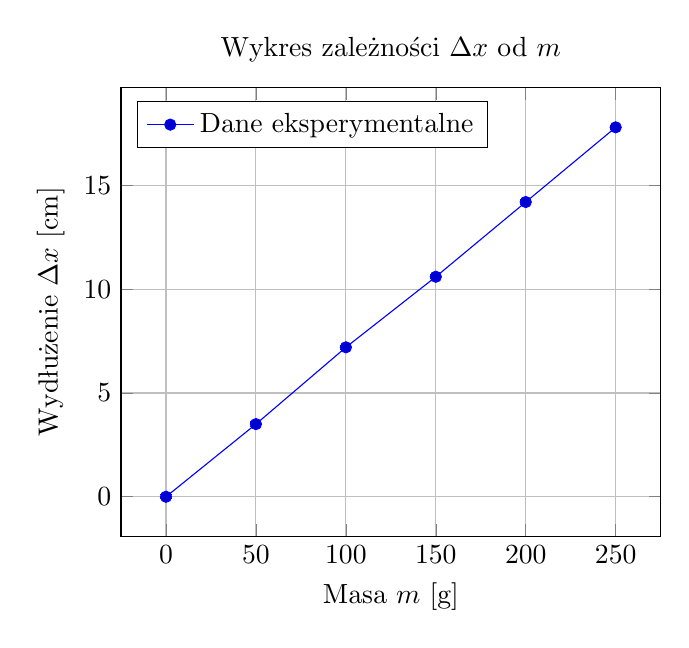
\begin{tikzpicture}
    \begin{axis}[
        ylabel={Wydłużenie $\Delta x$ [cm]}, % Etykieta osi X
        xlabel={Masa $m$ [g]},             % Etykieta osi Y
        grid=major,                        % Siatka na wykresie
        legend pos=north west,             % Pozycja legendy
        title={Wykres zależności $\Delta x$ od $m$}, % Tytuł wykresu
    ]
    \addplot+[
        mark=*,
        color=blue,
        error bars/.cd,
        y dir=both, % Enable error bars in both upward and downward directions
        y explicit % Explicitly define the errors
    ] coordinates {
        (0, 0.0) +- (0,0.1)
        (50, 3.5) +- (0,0.1)
        (100, 7.2) +- (0,0.1)
        (150, 10.6) +- (0,0.1)
        (200, 14.2) +- (0,0.1)
        (250, 17.8) +- (0,0.1)
    };
    \addlegendentry{Dane eksperymentalne}
    \end{axis}
\end{tikzpicture}



\begin{table}[h!]
\centering

\label{tab:coefficients}

\begin{tabular}{|c|c|c|}
\hline
\textbf{Masa \( m \) [kg]} & \textbf{Współczynnik kier. a} & \textbf{Odwrotność a czyli \( k \) [m/kg]} \\ 
\hline
0.050 & 0.74 & 1.351 \\ 
0.100 & 0.68 & 1.471 \\ 
0.150 & 0.72 & 1.389 \\ 
0.200 & 0.72 & 1.389 \\
\hline
\end{tabular}
\caption{Współczynniki kierunkowe \( k \) dla każdego przedziału pomiarowego}
\end{table}
\end{center}
}
\subsection{Wyznaczenie współczynnika sprężystości $k$}

Uśredniając wyniki z Tabeli 2 otrzymujemy:
{\large
\begin{equation}
    k = 1.400 \pm0.06 \frac{N}{m}
\end{equation}
}

\section{Dynamiczne wyznaczanie współczynnika sprężystości}
\subsection{Opis doświadczenia}
Druga metod wyznaczenia współczynnika sprężystości $k$ sprężyny opiera się na pomiarze okresu drgań wahadła $T$. Aby zwiększyć dokładność pomiaru, w ramach doświadczenie liczono czas, w jakim wahadło wykona 10 pełnych okresów. Dzięki temu zniwelować można błąd wynikający z szybkiego włączania i wyłączania stopera dla dużych częstości kołowych $\omega$ wahadła. Eksperyment przebiegał w następującej kolejności:
\begin{enumerate}
    \item Ciężarek wprawiono w ruch drgający w kierunku prostopadłym do podłoża.
    \item Stoperem zmierzono czas T 10 pełnych kresuów drgań.
    \item Zwiększono ciężar zawieszony na wahadle i powtórzono kroki (1) i (2).
\end{enumerate}
\subsection{Wyprowadzenie wzorów}

Za podstawowy wzór wyznaczenia współczynnika sprężystości posłuży wzór na okres drgań wahadła fizycznego:
{\large
\begin{equation}
    T = 2\pi\sqrt{\frac{m}{k}}
\end{equation}
}
Przekszałcając wzór (4) otrtzymujemy:
{\large
\begin{equation}
    k = \frac{4\pi^2m}{T^2}
\end{equation}
}
\subsection{Niepewność pomiarowa}
Niepewność pomiarową pomiaru czasu T okresu wyznaczymy na podstawie klasy wykorzystanego przedmiotu. Ponieważ stoper umożiwiał pomiar z dokładnością do 0.01 sekundy, zatem niepewność pomiarowa pomiaru okresu to $\Delta r_s = 0.01 [s]$. Masę ciężarków przyjmujemy za dokładną. Niepweność współczynnika kierunkowego $a$ wyznaczamy metodą graficzną w punkcie 3.5. 

\subsection{Wyniki pomiarów}
Wyniki pomiarów dla drugiej sprężyny przedstwiono w Tabeli 3:
\begin{table}[h!]
\centering
\begin{tabular}{|c|c|c|c|c|}
\hline
\textbf{Lp.} & \textbf{Masa[$g$]} & \textbf{Okres*10[$s$]} & \textbf{Okres[$s$]} & \textbf{Okres $T^2$}\\
\hline
1 & 0 & 0 & 0 & 0\\
2 & 500 & 9.11 & 0.911 & 0.823\\
3 & 450 & 8.59 & 0.859 & 0.737\\
4 & 400 & 8.04 & 0.804 & 0.646\\
5 & 350 & 7.56 & 0.756 & 0.571\\
6 & 300 & 7.12 & 0.712 & 0.507\\
\hline
\end{tabular}
\caption{Wyniki pomiarów}
\label{table:students}
\end{table}
\subsection{Wyniki doświadczenia}
Wyniki pomiarów zebrano na wykresie. Aby przedstawić, że współczynnik $k$ jest w przybliżeniu stały, os 0X została oznaczona jako $T^2$. 
\begin{center}
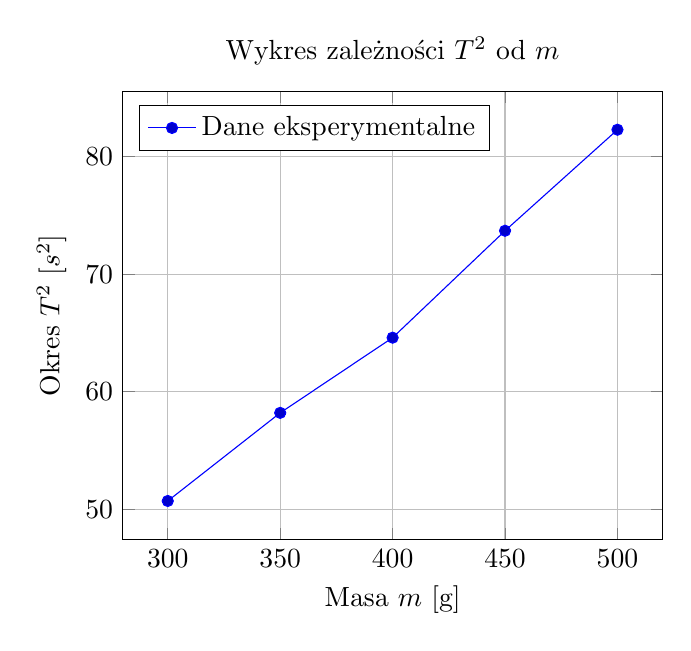
\begin{tikzpicture}
    \begin{axis}[
        ylabel={Okres $T^2$ [$s^2$]}, % Etykieta osi X
        xlabel={Masa $m$ [g]},             % Etykieta osi Y
        grid=major,                        % Siatka na wykresie
        legend pos=north west,             % Pozycja legendy
        title={Wykres zależności $T^2$ od $m$}, % Tytuł wykresu
    ]
    \addplot+[
        mark=*,
        color=blue,
        error bars/.cd,
        y dir=both, % Enable error bars in both upward and downward directions
        y explicit % Explicitly define the errors
    ] coordinates {
        (300, 50.7) +- (0,0.1)
        (350, 58.2) +- (0,0.1)
        (400, 64.6) +- (0,0.1)
        (450, 73.7) +- (0,0.1)
        (500, 82.3) +- (0,0.1)
    };
    \addlegendentry{Dane eksperymentalne}
    \end{axis}
\end{tikzpicture}

\end{center}
Korzystając z metody graficznej oraz wzoru (5) wyznaczamy współczynnik kierunowy wraz z niepewnością pomiarową. Współczynnik otrzymano jak iloraz różnicy pomiarów $T^2$ oraz mas (w tym przypadku równą zawsze 0.05 kg).
\begin{center}
    \begin{table}[h!]
\centering

\label{tab:coefficients}

\begin{tabular}{|c|c|}
\hline
\textbf{Masa \( m \) [kg]} & \textbf{Współczynnik kierunkowy \( a \) [$s^2/kg$]} \\ 
\hline
1 & 0.78 \\ 
2 & 0.67\\ 
3 & 0.54 \\ 
4 & 0.58 \\
\hline
\end{tabular}
\caption{Współczynniki kierunkowe \( k \) dla każdego przedziału pomiarowego}
\end{table}
\end{center}
Niepewność pomiarowa współczynnika kierunkowego zależała jedynie od $T$ i wyniosła $\Delta r_k = 0.02$
\subsection{Wyznaczenie współczynnika sprężystości $k$}
Ostatecznie uwzględniając stałą proporcjonalności $4\pi^2$ i dane z Tabeli 4 otzymujemy:
{\large
\begin{equation}
    k = 25.34\pm0.02N/m
\end{equation}
}
\section{Wyznaczenie modułu sztywności sprężyny}
\subsection{Opis doświadczenia}
Moduł sztywności $G$ to wielkość określająca sprężystość materiału przy rozciąganiu i ściskaniu. W tym przypadku wynaczenie modułu sprowadza się do pomiaru następujących wielkości:
\begin{enumerate}
    \item $r$ - promień drutu, z którego została wykonana sprężyna
    \item $N$ - liczba zwojów sprężyny
    \item $R$ - promień sprężyny
\end{enumerate}
\subsection{Wyprowadzenie wzorów}
Aby wyznaczyć moduł sztywności $G$ skorzystamy ze wzoru:
{\large
\begin{equation}
    k = \frac{Gr^2}{4NR^3}
\end{equation}
}
Po przekształceniach otrzymujemy:
{\large
\begin{equation}
    G = k\frac{4NR^3}{r^2}
\end{equation}
}
\subsection{Niepewność pomiarowa}
Niepewność pomiarową $u(f)$ wyznaczamy jako niepewność wielkości złożonej. Niepewność każdego pomiaru to $\Delta r = 0.001[m]$Pochodne cząstkowe względem $r, N$ i $R$ wynoszą odpowiednio:
{\large
\begin{equation}
    \frac{\partial G}{\partial r} = -\frac{8kNR^3}{r^3} = A
\end{equation}

\begin{equation}
    \frac{\partial G}{\partial N} = \frac{4kR^3}{r^2} = B
\end{equation}

\begin{equation}
    \frac{\partial G}{\partial R} = \frac{12kNR^2}{r^2} = C
\end{equation}
}
Ostatecznie wzór na niepewność pomiarową przyjmuje postać:
{\large
\begin{equation}
    u(f) = \sqrt{(A\Delta r)^2+(B\Delta r)^2+(C\Delta r)^2}
\end{equation}
}
gdzie $A, B$ i $C$ to wartości poszczególnych pochodnych cząstkowych, a $k$ to współczynnik sprężystości.
\subsection{Wyniki pomiarów}
Wyniki pomiarów zebrano w Tabeli 5:
\begin{center}
\begin{table}[h!]
\centering
\label{tab:coefficients}
\begin{tabular}{|c|c|c|}
\hline
\textbf{Promień drutu \( r \) [mm]} & \textbf{Liczba zwojów \( N \) [*]} &\textbf{Promień sprężyny $R$[mm]}\\ 
\hline
0.435 & 81 & 5.2 \\
\hline
\end{tabular}
\caption{Wyniki pomiarów własności sprężyny}
\end{table}
\end{center}
\subsection{Wyznaczenie modułu sztywności}
Aby wyznaczyć moduł sztywności sprężyny dane z Tabeli 5 wstaiamy do wzoru (7). Niepewność wyznaczamy podstawiając te same dane do wzorów (8), (9), (10) i (11).
{\large
\begin{equation}
    G=353.106\pm0.027N/m^2
\end{equation}
}

\begin{comment}
\subsection{Opis doświadczenia}
\subsection{Wyprowadzenie wzorów}
\subsection{Niepewność pomiarowa}
\subsection{Wyniki pomiarów}
\subsection{Wyniki doświadczenia}
\subsection{Wyznaczenie współczynnika sprężystości $k$}
\end{comment}
\end{document}